%%%%%%%%%%%%%%%%%%%%%%%%%%%%%%%%%%%%%%%%%%%%%%%%%%%%%%%%%%%%%%%%%%%
\section{Descripci�n} 
Desarrollar un programa \texttt{BolaMovil.java} que muestre en pantalla una ventana
rectangular con fondo de color azul sobre la que se ver� un c�rculo centrado en la ventana
y un panel con cuatro botones que permiten mover el c�rculo hacia arriba, abajo, izquierda
y derecha.


%%%%%%%%%%%%%%%%%%%% Fig. %%%%%%%%%%%%%%%%%%%%%%%%%%%%%%%%%%%
\begin{figure}[h]
\centerline{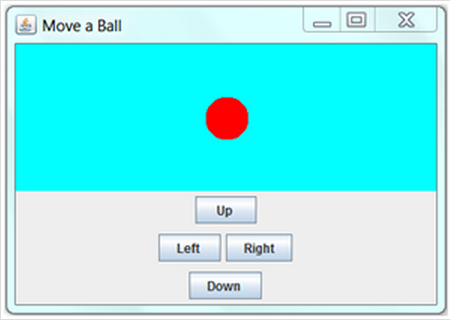
\includegraphics[width=0.5\linewidth]{bola}}
\caption{Interfaz gr�fica del programa} 
\label{fig:bola} 
\end{figure}
%%%%%%%%%%%%%%%%%%%%%%%%%%%%%%%%%%%%%%%%%%%%%%%%%%%%%%%%%%%%%%
La Figura \ref{fig:bola} muestra un ejemplo al que deber�a parecerse la salida del programa a elaborar.


Las siguientes deben tomarse como especificaciones de la aplicaci�n a desarrollar:
\begin{itemize}
\item Utilizando \texttt{AssertJ}, desarrolle tests unitarios que aseguren que el comportamiento del progama
      es el deseado.
\item Utilice tambi�n \texttt{JaCoCo} para analizar el cubrimiento que los tests unitarios realizan sobre el
      c�digo desarrollado.
\item La interfaz contendr� los cuatro botones: \texttt{Arriba}, \texttt{Abajo}, \texttt{Izquierda}, \texttt{Derecha}
      cuyas funciones ya se han comentado.
\item Cuando el c�rculo alcanza cualquiera de los bordes de la ventana, se ha de impedir
      su movimiento en la direcci�n del borde alcanzado (los bordes son impenetrables).
\item El n�mero de pixeles que se desplaza el c�rculo por la ventana con cada pulsaci�n de un bot�n
      ser� un par�metro que el programa ha de leer en l�nea de comandos.
\item Si el programa se ejecuta sin pasar ning�n par�metro en l�nea de comandos, se debe escribir
      un mensaje en la consola indicando la forma correcta de ejecuci�n del programa.
\item Se valorar� positivamente que el dise�o sea efectivamente orientado a objetos, modelando con diferentes
      clases los distintos elementos que intervienen en la aplicaci�n.
\item El programa que aqu� se propone se tomar� como punto de partida para desarrollar una aplicaci�n similar
      a la que aqu� se propone. 
      As� pues, ser� beneficioso el realizar un dise�o muy modular y flexible.
\item Evite utilizar clases o m�todos que no hayan sido explicados en las clases de teor�a.
\end{itemize}
%%%%%%%%%%%%%%%%%%%%%%%%%%%%%%%%%%%%%%%%%%%%%%%%%%%%%%%%%%%%%%%%%%%
